\documentclass[12pt]{article}

\usepackage{report}

\usepackage[utf8]{inputenc} % allow utf-8 input
\usepackage[T1]{fontenc}    % use 8-bit T1 fonts
\usepackage[colorlinks=true, linkcolor=black, citecolor=blue, urlcolor=blue]{hyperref}       % hyperlinks
\usepackage{url}            % simple URL typesetting
\usepackage{booktabs}       % professional-quality tables
\usepackage{amsfonts}       % blackboard math symbols
\usepackage{nicefrac}       % compact symbols for 1/2, etc.
\usepackage{microtype}      % microtypography
\usepackage{lipsum}		% Can be removed after putting your text content
\usepackage{graphicx}
\usepackage{natbib}
\usepackage{doi}
\usepackage{listings}
\usepackage{xcolor}
\usepackage{float}
\setcitestyle{aysep={,}}



\title{Step 1: 1-bit Operations}

\author{Connor Nauert, Daniel Okoh, James Webb\\
\AND\\
\AND
\AND
\AND
\AND
	CS.3339 Computer Architecture\\
\AND
	Texas State University\\
}

\date{September 17, 2026}

\renewcommand{\headeright}{1-bit Operations - Blue Giraffes}
\renewcommand{\undertitle}{Blue Giraffes}
\renewcommand{\shorttitle}{}

\definecolor{codegreen}{rgb}{0,0.6,0}
\definecolor{codegray}{rgb}{0.5,0.5,0.5}
\definecolor{codepurple}{rgb}{0.58,0,0.82}
\definecolor{backcolour}{rgb}{0.95,0.95,0.92}

\lstdefinestyle{mystyle}{
    backgroundcolor=\color{backcolour},   
    commentstyle=\color{codegreen},
    keywordstyle=\color{magenta},
    numberstyle=\tiny\color{codegray},
    stringstyle=\color{codepurple},
    basicstyle=\ttfamily\footnotesize,
    breakatwhitespace=false,         
    breaklines=true,                 
    captionpos=b,                    
    keepspaces=true,                 
    numbers=left,                    
    numbersep=5pt,                  
    showspaces=false,                
    showstringspaces=false,
    showtabs=false,                  
    tabsize=2
}

\lstset{style=mystyle}


\begin{document}
\maketitle

\newpage
\thispagestyle{empty}


\newpage
\setcounter{page}{1}
\section{Introduction}
In this project, we are designing a small computer from scratch by using Verilog for
hardware programming. We will also be using GTKWave to analyze test case waveforms and
display the inputs and outputs of the gates.

Step 1 involves constructing the initial simple 1-bit circuits.

\section{Verilog Code}
\label{sec:headings}

In this section, we will go over every circuit and the associated Verilog code for each one, including the test modules.

\subsection{Not Circuit}
The Not circuit is the most simple of the 1-bit gates. One input, A, is inverted to an output X. If A is a 1, X will be a 0. If A is 0, X will be a 1.
\lstinputlisting[language=Verilog]{Verilog/not_test.v}

Testing the Not circuit involves creating a register A and measuring an output X. There are two possible states to be tested: when A is 0 and when A is 1.
The pound symbol in the snippet below calls for the computer to wait for some amount of nanoseconds, which allows us to observe how the gate acts
over time.
\lstinputlisting[language=Verilog]{Verilog/not_tb.v}

\subsection{Nand Circuit}
The Nand circuit is composed of a Not gate and an And gate. Two inputs, A and B, are inputted into an And gate. The output of the And gate is then inverted and outputted to X.
This means that if A and B are both 1, the And gate will invert the combined 1 into a 0. The other three states will output a 1.
\lstinputlisting[language=Verilog]{Verilog/nand_test.v}

To test the Nand circuit, we have created two registers, A and B, as well as a wire X. This way we are able to take two inputs at a time and test each possible input for the circuit. If it's working correctly, X should be equal to 1 for all inputs except when both A and B are equal to 1.
\lstinputlisting[language=Verilog]{Verilog/nand_tb.v}

\begin{figure}[h]
    \centering
    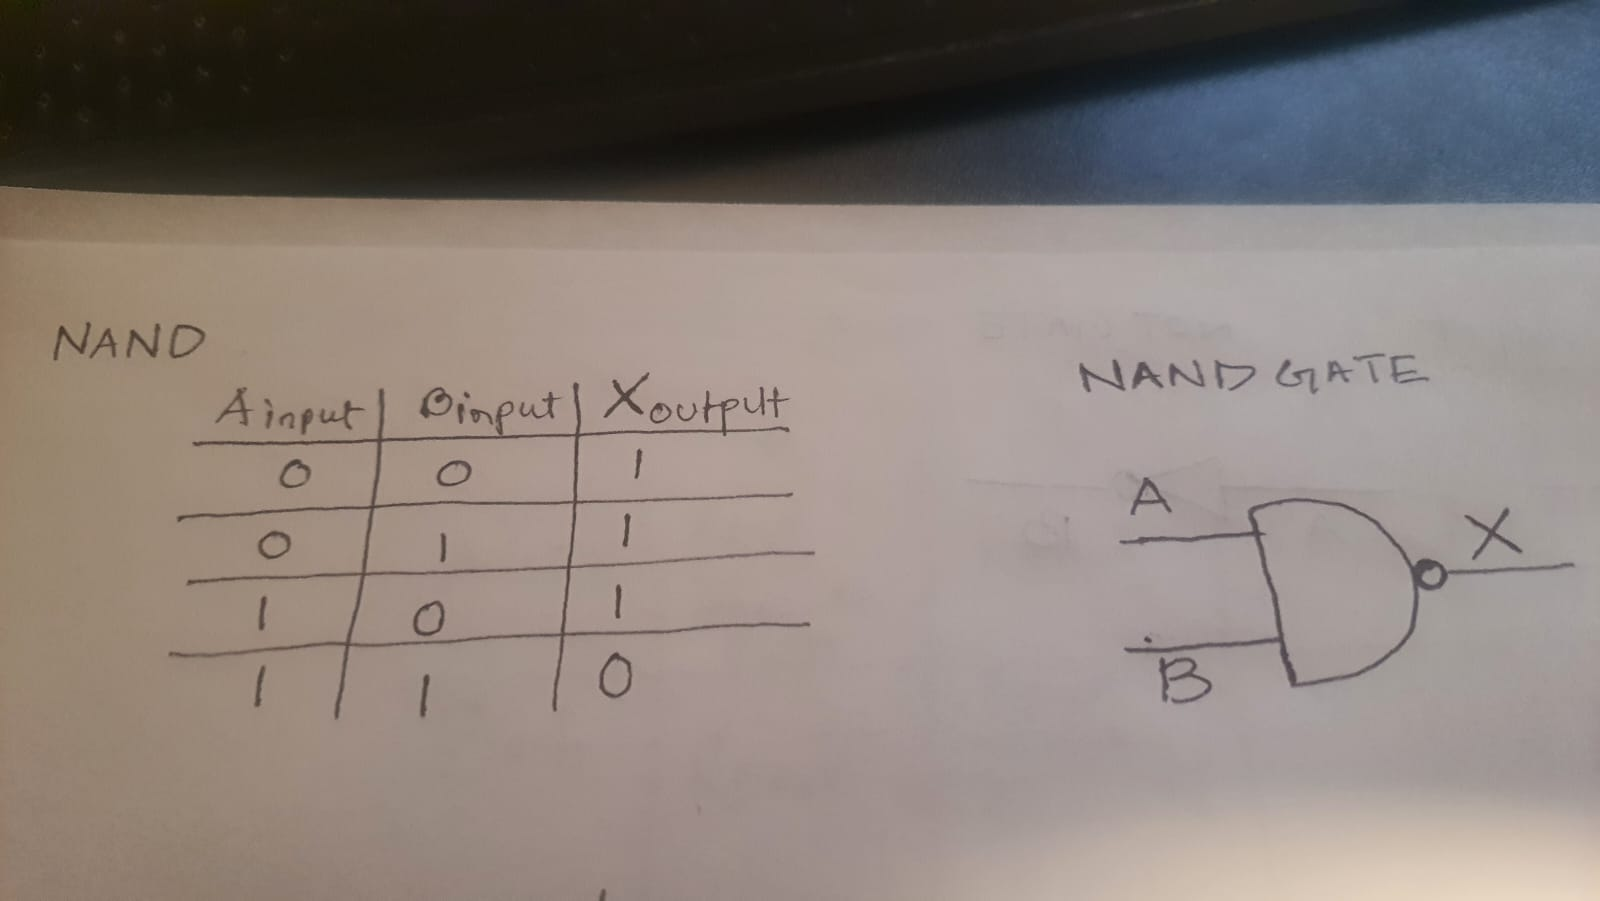
\includegraphics[width = 1.0\textwidth]{figs/NAND_IMG.jpg}
    \caption{Nand truth table and gate}
    \label{fig:enter-label}
\end{figure}

\newpage

\subsection{Nor Circuit}
The Nor circuit is similar to the Nand circuit in that it is the inverse of another gate. The Or gate will take two inputs, A and B.
The Not gate will switch the bit outputted by the Or gate, which is then wired to X. If both A and B are 0, then X should be 1. Otherwise,
X is 0.
\lstinputlisting[language=Verilog]{Verilog/nor_test.v}

The Nor circuit testbench also uses two inputs, one output, and four possible states.
\lstinputlisting[language=Verilog]{Verilog/nor_tb.v}

\subsection{1x4 Arithmetic Shift Circuit}
The Arithmetic Shift circuit will take a 4-bit pattern, and \emph{shift} them over to the left or to the right one bit. Due to this shifter being
arithmetic, new bits will be zeros unless shifting we a negative integer to the right. Negative numbers will be sign-extended, and new bits will
be ones.

We implement this by using an array of 4-bit registers as input, which is then mapped to a 4-bit wire output. We also use a \emph{dir} register to
specify the direction of the shift.
\lstinputlisting[language=Verilog]{Verilog/bitshift.v}

This testbench will set a 4-bit pattern, shift to the left, shift to the right, and repeat. For example, a pattern of 1001 shifted to the left would be 0010,
and a pattern of 1010 shifted to the right would be 1101.

\lstinputlisting[language=Verilog]{Verilog/bitshift_tb.v}


\section{Waveform Tests}

Now, we will showcase waveforms created by testing our four circuits. All waves were generated by vvp and rendered with GTKWave.

\subsection{Not Circuit Waveform}

In the first half of the waveform, our input (A) is 0, or low. This is inverted to 1 (high) in the output X.
After 20ns, A is flipped to 1 and X changes accordingly to 0.

\begin{figure}[h]
    \centering
    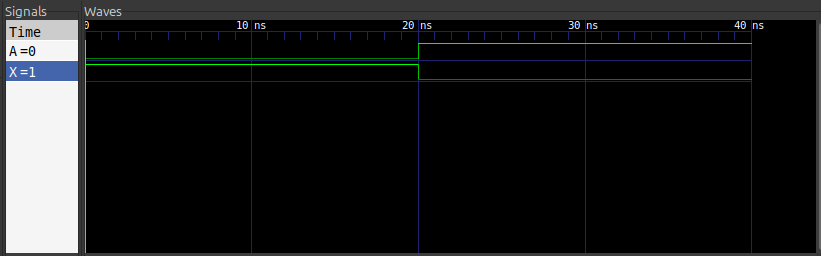
\includegraphics[width = 1.0\textwidth]{figs/not_waveform.png}
    \caption{Not circuit waveform. There are two sections since there are two states.}
\end{figure}

\subsection{Nand Circuit Waveform}

test

\begin{figure}[h]
    \centering
    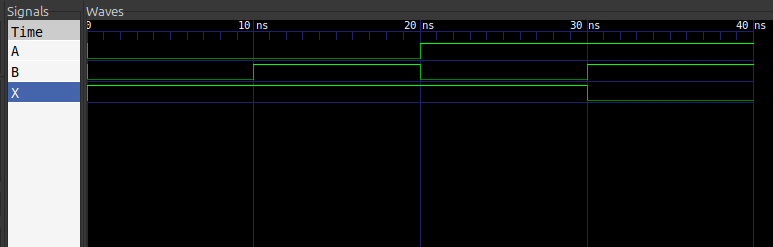
\includegraphics[width = 1.0\textwidth]{figs/nand_waveform.png}
    \caption{Nand circuit waveform. Notice we now have four states.}
\end{figure}

\subsection{Nor Circuit Waveform}

test

\begin{figure}[h]
    \centering
    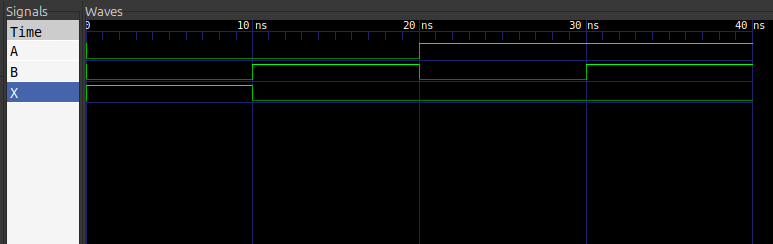
\includegraphics[width = 1.0\textwidth]{figs/nor_waveform.png}
    \caption{Nor circuit waveform.}
\end{figure}

\subsection{1x4 Arithmetic Shifter Waveform}

test

\begin{figure}[h]
    \centering
    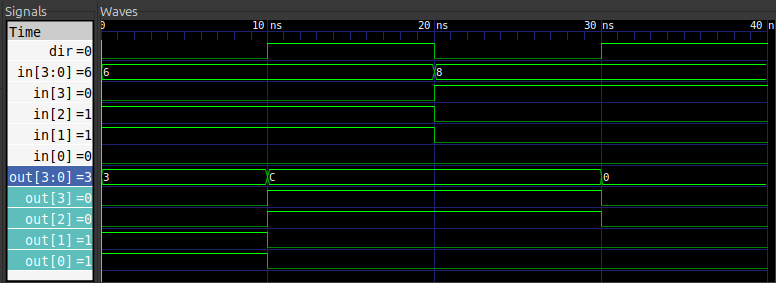
\includegraphics[width = 1.0\textwidth]{figs/bitshift.png}
    \caption{Arithmetic shifter waveforms, with a DIR register and 8 bits.}
\end{figure}

\section{Conclusion}

In conclusion,

\end{document}



